\documentclass[11pt,letterpaper]{article}
\usepackage[lmargin=1in,rmargin=1in,tmargin=1in,bmargin=1in]{geometry}
\usepackage{../style/homework}
\usepackage{../style/commands}
\setbool{quotetype}{false} % True: Side; False: Under
\setbool{hideans}{false} % Student: True; Instructor: False

% -------------------
% Content
% -------------------
\begin{document}

\homework{8: Due 03/06}{Laura, clear out the rest of my day! I have to push a boulder up a hill and then have it roll over me time and time again with no regard for my well-being.}{Princess Carolyn, BoJack Horseman}

% Problem 1
\problem{10} Kelsey is gambling at a casino. She is playing a game where you roll two die. If you roll two 6's, you win \$100. If you the dice and the numbers on both die are four or greater (but not two 6's), you win \$10. If the numbers on both die are less than 3, you lose \$8. Otherwise, you win nothing. You must pay \$5 as a `buy-in' each round to play. Find the amount that you win/lose `on average.' Should one play this game? \pspace

\sol Rolling two die, there are $6 \cdot 6= 36$ total outcomes for the values on the two die. There is only one way to roll two 6's---by rolling two 6's. If you want to roll a four or bigger on each die, there are 3 possibilities for each die (4, 5, or 6) so that there are $3 \cdot 3= 9$ such combinations. But this includes two 6's on each die. Therefore, there are $9 - 1= 8$ total ways to roll the dice and have a four or greater on each die. If a number on a die is less than 3, there are 2 possibilities (1 or 2). Therefore, there are $2 \cdot 2= 4$ total combinations where both numbers on the die are less than 3. But then we have\dots
	\[
	\begin{aligned}
	P(\text{two 6's})&= \dfrac{1}{36} \\[0.3cm]
	P(\text{Four or Great (Not Boxcars)})&= \dfrac{8}{36}= \dfrac{2}{9} \\[0.3cm]
	P(\text{Less than 3})&= \dfrac{4}{36}= \dfrac{1}{9} \\[0.3cm]
	P(\text{Anything Else})&= 1 - \dfrac{1}{36} - \dfrac{8}{36} - \dfrac{4}{36}= \dfrac{23}{36}
	\end{aligned}
	\]
We can create a table of the possible outcomes, their probability, and their net expected payout (that is, the payout minus the \$5 fee to play). We have\dots \par
	\begin{table}[!ht]
	\centering
	\begin{tabular}{|l|c|c|c|c|} \hline
	Outcome & Two 6's & Four or Greater (Not Boxcars) & Less than 3 & Anything Else \\ \hline 
	Probability & $\dfrac{\stackrel{\phantom{1}}{1}}{36}$ & $\dfrac{2}{9}$ & $\dfrac{1}{9}$ & $\dfrac{23}{36}$ \\[0.3cm] \hline
	Value & \$95 & \$5 & $-$\$13 & $-$\$5 \\ \hline
	\end{tabular}
	\end{table} \par
We can then compute the expected payout:
	\[
	EX= \sum x P(x)= \$95 \cdot \dfrac{1}{36} + \$5 \cdot \dfrac{2}{9} - \$13 \cdot \dfrac{1}{9} - \$5 \cdot \dfrac{23}{36} \approx \$2.639 + \$1.111 - \$1.444 - \$3.194= -\$0.888 \approx -\$0.89
	\]
Because the expected value is negative, on average, you lose \$0.89 each game by playing this game. Therefore, you should not play this game. 



\newpage



% Problem 2
\problem{10} Find the least square regression line for the points: $(1, 3), (3, 5), (1, 2), (2, 2)$. Show all your work. \pspace

\sol First, observe that we have $n= 4$ points. Examining the $x$ and $y$ values, we have\dots
	\[
	\begin{aligned}
	\overline{x}&= \dfrac{1 + 3 + 1 + 2}{4}= \dfrac{7}{4} \approx 1.75 \\[0.3cm]
	\overline{y}&= \dfrac{3 + 5 + 2 + 2}{4}= \dfrac{12}{4}= 3
	\end{aligned}
	\]
But then we have\dots \par
	\begin{table}[!ht]
	\centering
	\begin{tabular}{rrrrrrr}
	\multicolumn{1}{r|}{$x_i$} & \multicolumn{1}{|r|}{$y_i$} & \multicolumn{1}{|r|}{$x_i - \overline{x}$} & \multicolumn{1}{|r|}{$(x_i - \overline{x})^2$} & \multicolumn{1}{|r|}{$y_i - \overline{y}$} & \multicolumn{1}{|r|}{$(y_i - \overline{y})^2$} & \multicolumn{1}{|r}{$(x_i - \overline{x})(y_i - \overline{y})$} \\ \hline
	\multicolumn{1}{r|}{$1$} & \multicolumn{1}{|r|}{$3$} & \multicolumn{1}{|r|}{$-0.75$} & \multicolumn{1}{|r|}{$0.5625$} & \multicolumn{1}{|r|}{$0$} & \multicolumn{1}{|r|}{$0$} & \multicolumn{1}{|r}{$0$} \\ 
	\multicolumn{1}{r|}{$3$} & \multicolumn{1}{|r|}{$5$} & \multicolumn{1}{|r|}{$1.25$} & \multicolumn{1}{|r|}{$1.5625$} & \multicolumn{1}{|r|}{$2$} & \multicolumn{1}{|r|}{$4$} & \multicolumn{1}{|r}{$2.5$} \\
	\multicolumn{1}{r|}{$1$} & \multicolumn{1}{|r|}{$2$} & \multicolumn{1}{|r|}{$-0.75$} & \multicolumn{1}{|r|}{$0.5625$} & \multicolumn{1}{|r|}{$-1$} & \multicolumn{1}{|r|}{$1$} & \multicolumn{1}{|r}{$0.75$} \\ 
	\multicolumn{1}{r|}{$2$} & \multicolumn{1}{|r|}{$2$} & \multicolumn{1}{|r|}{$0.25$} & \multicolumn{1}{|r|}{$0.0625$} & \multicolumn{1}{|r|}{$-1$} & \multicolumn{1}{|r|}{$1$} & \multicolumn{1}{|r}{$-0.25$} \\ \hline
	& & Total: & $2.75$ & Total: & $6$ & $3$
	\end{tabular}
	\end{table}
But then we have\dots
	\[
	\begin{aligned}
	\hspace{-0.3cm} s_x^2&= \dfrac{1}{n - 1} \sum (x_i - \overline{x})^2= \dfrac{1}{3} \cdot 2.75= 0.916667 \Longrightarrow s_x= \sqrt{0.916667}= 0.957427 \\[0.3cm]
	\hspace{-0.3cm} s_y^2&= \dfrac{1}{n - 1} \sum (y_i - \overline{y})^2= \dfrac{1}{3} \cdot 6= 2 \Longrightarrow s_y= \sqrt{2}= 1.41421 \\[0.3cm]
	\hspace{-0.3cm} r&= \dfrac{1}{n - 1} \sum \left( \dfrac{x_i - \overline{x}}{s_x} \right) \left( \dfrac{y_i - \overline{y}}{s_y} \right)= \dfrac{1}{n - 1} \cdot \dfrac{1}{s_x} \cdot \dfrac{1}{s_y} \sum (x_i - \overline{x})(y_i - \overline{y})= \dfrac{1}{3} \cdot \dfrac{1}{0.957427} \cdot \dfrac{1}{1.41421} \cdot 3= 0.738551
	\end{aligned}
	\]
This allows us to compute the coefficients for our model:
	\[
	\begin{aligned}
	b_1&= r \, \dfrac{s_y}{s_x}= 0.738551 \cdot \dfrac{1.41421}{0.957427}= 1.09091 \\[0.3cm]
	b_0&= \overline{y} - b_1 \overline{x}= 3 - 1.09091 (1.75)= 1.09091
	\end{aligned}
	\]
Therefore, the least square regression line is\dots
	\[
	\widehat{y}= b_1x + b_0= 1.09091x + 1.09091
	\]
This linear regression has $r^2$ value $0.545458$ and is shown with the data points below: 
	\[
	\fbox{
	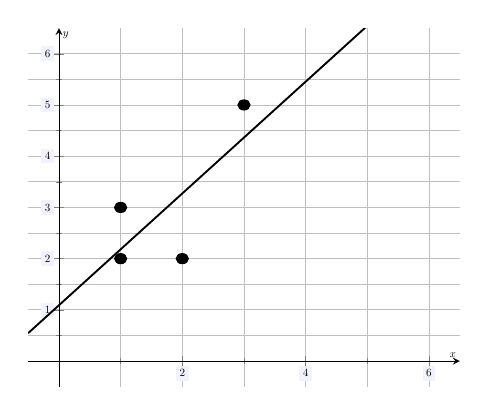
\begin{tikzpicture}[scale=0.8,every node/.style={scale=0.5}]
	\begin{axis}[
	grid=both,
	axis lines=middle,
	ticklabel style={fill=blue!5!white},
	xmin= -0.5, xmax=6.5,
	ymin= -0.5, ymax=6.5,
	xtick={0,2,...,16},
	ytick={0,1,...,6},
	minor x tick num = 1,
	minor y tick num = 1,
	xlabel=\(x\),ylabel=\(y\),
	]
	\addplot[domain=-0.5:6.5,samples=2,line width=0.03cm] (x, 1.09091*x + 1.09091);
	
	\draw[fill=black] (1,3) circle (0.1);
	\draw[fill=black] (3,5) circle (0.1);
	\draw[fill=black] (1,2) circle (0.1);
	\draw[fill=black] (2,2) circle (0.1);
	\end{axis}
	\end{tikzpicture}
	}
	\] 



\newpage



% Problem 3
\problem{10} Given the following information below, find the least square regression line. Show all your work. 
	\[
	\begin{aligned}
	n&= 200 \\
	\overline{x}&= 4.42726, \quad \sigma_x^2&= 10.6639 \\
	\overline{y}&= 46.5248, \quad \sigma_y^2&= 1053.77 \\
	R&= 0.962639
	\end{aligned}
	\] \pspace

\sol We have\dots
	\[
	\begin{aligned}
	\sigma_x^2&= 10.6639 \Longrightarrow \sigma_x= \sqrt{10.6639}= 3.26556 \\[0.3cm]
	\sigma_y^2&= 1053.77 \Longrightarrow \sigma_y= \sqrt{1053.77}= 32.4618 
	\end{aligned}
	\]
But then we can compute the model coefficients:
	\[
	\begin{aligned}
	b_1&= r \, \dfrac{\sigma_y}{\sigma_x}= 0.962639 \cdot \dfrac{32.4618}{3.26556}= 9.56926 \\[0.3cm]
	b_0&= \overline{y} - b_1 \overline{x}= 46.5248 - 9.56926(4.42726)= 4.1592
	\end{aligned}
	\]
Therefore, the least square regression line is\dots
	\[
	\widehat{y}= b_1x + b_0= 9.56926x + 4.1592
	\]



\newpage



% Problem 4
\problem{10} Match each regression coefficient to its corresponding graph. 
	\begin{figure}[!ht]
	\centering
	\begin{minipage}{0.45\textwidth}
	   \centering
	   \includegraphics[width=0.9\textwidth]{reg1.png}
	   \caption*{(a)}
	\end{minipage}\hfill
	\begin{minipage}{0.45\textwidth}
	   \centering
	   \includegraphics[width=0.9\textwidth]{reg2.png}
	   \caption*{(b)}
	\end{minipage}
	\begin{minipage}{0.45\textwidth}
	   \centering
	   \includegraphics[width=0.9\textwidth]{reg3.png}
	   \caption*{(c)}
	\end{minipage}
	\begin{minipage}{0.45\textwidth}
	   \centering
	   \includegraphics[width=0.9\textwidth]{reg4.png}
	   \caption*{(d)}
	\end{minipage}
	\end{figure}

\begin{enumerate}[(i)]
\item \usol{0.25cm}{(b)}: $R= 0.836288$
\item \usol{0.25cm}{(c)}: $R= -0.998836$
\item \usol{0.25cm}{(d)}: $R= 0.997066$
\item\usol{0.25cm}{(a)}: $R= -0.759531$
\end{enumerate} 


\end{document}